\documentclass[twocolumn]{article}
\usepackage[margin=1in]{geometry}
\usepackage{tikz}
\usetikzlibrary{arrows.meta,positioning}
\begin{document}
\section{Mechanism}
The figure is deliberately wider than one column.
\begin{figure}[ht]
\centering
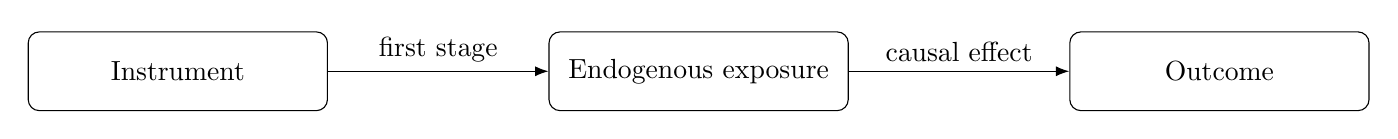
\begin{tikzpicture}[
  box/.style={draw, rounded corners, minimum width=38mm, minimum height=10mm},
  node distance=28mm,
  >=Latex
]
\node[box] (a) {Instrument};
\node[box, right=of a] (b) {Endogenous exposure};
\node[box, right=of b] (c) {Outcome};
\draw[->] (a) -- node[above] {first stage} (b);
\draw[->] (b) -- node[above] {causal effect} (c);
\end{tikzpicture}
\caption{A diagram that fits poorly in one column.}
\end{figure}
\end{document}
